\subsection{球缺的体积}\label{subsec:2-13}
\begin{enhancedline}

我们常见到钢桥、轮船、锅炉上有圆头的铆钉,铆钉的圆头具有球缺的形象。
一个球被平面截下的一部分叫做\zhongdian{球缺}。截面叫做\zhongdian{球缺的底面},
垂直于截面的直径被截下的线段长叫做\zhongdian{球缺的高}(图 \ref{fig:ltjh-2-73})。

\begin{wrapfigure}[6]{r}{5.5cm}
    \centering
    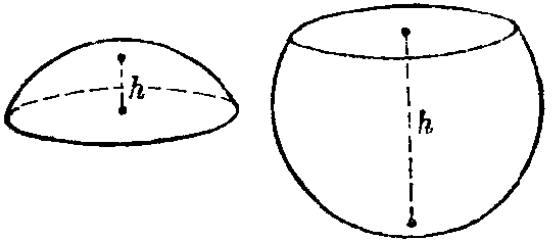
\includegraphics[width=5cm]{../pic/ltjh-ch2-73.png}
    \caption{}\label{fig:ltjh-2-73}
\end{wrapfigure}

显然,球缺也可以看做是球冠和截面所围成的几何体。
球缺的体积公式,可仿球的体积求法推出。设球的半径是 $R$,球缺的高是 $h$。
利用前节的图 \ref{fig:ltjh-2-72},因为已证明了平行于平面 $\alpha$ 的任意截面面积都分别相等,
所以根据\hyperref[zgyl]{祖暅原理},球缺的体积
\begin{align*}
    V_\text{球缺} &= V_{\text{圆柱} LKNP} - V_{\text{圆台} LABP} \\
        &= \pi R^2h - \exdfrac{1}{3} \pi h[R^2 + R(R - h) + (R - h)^2] \\
        &= \pi Rh^2 - \exdfrac{1}{3} \pi h^3 \\
        &= \exdfrac{1}{3} \pi h^2 (3R - h)
\end{align*}

由此我们得到下面的定理:

\begin{dingli}[定理][qiuque-tj]
    如果球的半径是 $\bm{R}$,球缺的高是 $\bm{h}$,那么球缺的体积是
    \begin{center}
        \framebox[14em]{$\bm{V_\text{球缺} = \exdfrac{1}{3} \pi h^2 (3R - h)}$。}
    \end{center}
\end{dingli}

这个公式对于求半球,大于半球的球缺,整个球的体积都适用,例如,
用 $R$ 代 $h$,就得到半球的体积与 $\exdfrac{2}{3} \pi R^3$。


\liti 钢铆钉钉头呈球缺形,钉身呈圆柱形,尺寸如图 \ref{fig:ltjh-2-74}(单位:mm)。
已知钢的比重是 $7.8\;\kmlflm$,求铆钉的重量(精确到 1 g)。

\jie 钉头的体积是
\begin{align*}
    V_\text{球缺} &= \exdfrac{1}{3} \pi h^2 (3R - h) \\
        &= \exdfrac{1}{3} \times 3.14 \times 6^2 \times (3 \times 10 - 6) \\
        &\approx 904 \;(\lfhm) \juhao
\end{align*}

钉身的体积是
\begin{align*}
    V_\text{圆柱} &= \pi R_1^2 h_1 \\
        &= 3.14 \times 5^2 \times 20 \\
        &\approx 1570 \;(\lfhm) \juhao
\end{align*}
所以铆钉的重量是 \quad $7.8 \times \dfrac{904 + 1570}{1000} \approx 19 \; (\ke)$。

答:铆钉的重量约 19 g。

\begin{figure}[htbp]
    \centering
    \begin{minipage}[b]{7cm}
        \centering
        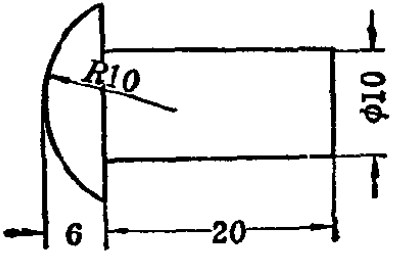
\includegraphics[width=5cm]{../pic/ltjh-ch2-74.png}
        \caption{}\label{fig:ltjh-2-74}
    \end{minipage}
    \qquad \qquad
    \begin{minipage}[b]{7cm}
        \centering
        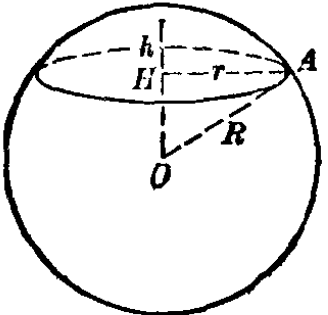
\includegraphics[width=4cm]{../pic/ltjh-ch2-75.png}
        \caption{}\label{fig:ltjh-2-75}
    \end{minipage}
\end{figure}

\liti 已知:球缺底面半径是 $r$,高是 $h$。 求证:球缺的体积是
\zhongdian{$$ \bm{V_\text{球缺} = \exdfrac{1}{6} \pi h (3r^2 + h^2)} \juhao $$}

\zhengming 设截得球缺的球的半径是 $R$,由直角三角形 $OAH$ (图 \ref{fig:ltjh-2-75}),

\begin{gather*}
    r^2 = R^2 - (R - h)^2 = 2hR - h^2 \douhao \\
    R = \dfrac{r^2}{2h} + \exdfrac{h}{2} \juhao
\end{gather*}

代入球缺体积公式,得
\begin{align*}
    V_\text{球缺} &= \pi h^2 \left( \dfrac{r^2}{2h} + \exdfrac{h}{2} - \exdfrac{h}{3} \right) \\
        &= \exdfrac{1}{6} \pi h (3r^2 + h^2) \juhao
\end{align*}

在生产和生活中所遇到的物体,形状虽然比较复杂,但是很多都可以看作是由柱体、锥体、台体、
球体、球缺等组合(例如铆钉)或切割(例如螺帽)而成的。 所以,我们能求这些几何体的体积,
就能求那些形状比较复杂的物体的体积。 然而,更复杂的体积,例如环体的体积,还要在以后用积分法去解决。


\begin{lianxi}

\xiaoti{球缺的高是球的直径的 $\dfrac{1}{10}$。求它们体积的比。}

\xiaoti{球缺的底面半径是球的半径的 $\exdfrac{1}{2}$。体积是球的几分之几?}

\end{lianxi}

\end{enhancedline}

